\documentclass[11pt,a4paper]{article}

% ---------------------------------------------------------------- packages
\usepackage[T1]{fontenc}
\usepackage[utf8]{inputenc}
\usepackage{mathptmx}
\usepackage[a4paper,margin=2.5cm]{geometry}
\usepackage{amsmath,amssymb,amsthm,mathtools,bm}
\usepackage{graphicx,booktabs,array,tabularx,longtable,enumitem,xcolor}
\usepackage[font=small,labelfont=bf,format=hang]{caption}
\usepackage{siunitx}
\usepackage[section]{placeins}
\usepackage{fancyhdr}
\usepackage{microtype}
\usepackage[numbers,sort&compress]{natbib}
\usepackage[hidelinks,pdftitle={Statistical Mechanics of Molecular Adsorption on Interstellar Dust Grains},pdfauthor={Student Name}]{hyperref}
\usepackage[nameinlink,capitalise]{cleveref}

\sisetup{detect-all=true,per-mode=symbol,group-separator={\,},group-minimum-digits=4}
\setlength{\emergencystretch}{2em}
\setlength{\parskip}{0.45em}
\setlength{\parindent}{0pt}
\renewcommand{\arraystretch}{1.12}
\setlist{itemsep=0.1em,topsep=0.3em}
\captionsetup{skip=6pt}

% auto-generated numbers (code/make_figures.py)
\newcommand{\numentCanSmall}{2.76}
\newcommand{\numentCanLarge}{7.61}
\newcommand{\numentGCLarge}{15.60}
\newcommand{\numTdesOneYr}{26.7}
\newcommand{\numTdesTenGyr}{17.7}
\newcommand{\numTstir}{25.02}
\newcommand{\nummuKstir}{-1228}
\newcommand{\numbhwstir}{2.3979}
\newcommand{\numbmustir}{-49.09}
\newcommand{\numepsK}{1200}
\newcommand{\numhwK}{60}
\newcommand{\numepsJ}{1.657\times10^{-20}}
\newcommand{\numepsEV}{0.103}
\newcommand{\numhwJ}{8.284\times10^{-22}}
\newcommand{\numnuHz}{1.25}
\newcommand{\nummuJ}{-1.696\times10^{-20}}
\newcommand{\numlamT}{0.66}
\newcommand{\numngas}{1668}
\newcommand{\numtdesRep}{21}
\newcommand{\numlamsite}{0.4286}
\newcommand{\numzvRep}{1.3310}
\newcommand{\numnbarmode}{0.100}
\newcommand{\numdevNkilo}{-0.108}
\newcommand{\numdevQmega}{6.67e-06}
\newcommand{\numdevNmega}{1.72e-06}
\newcommand{\numrelQpred}{1.11e-06}
\newcommand{\numslopeQ}{-1.000}
\newcommand{\numslopeN}{-0.998}
\newcommand{\numnchecks}{27}
\newcommand{\numnpass}{27}
\newcommand{\numrelfluctN}{1.53e-03}
\newcommand{\numsighsq}{0.3300}
\newcommand{\numthetaRep}{0.30}
\newcommand{\numrsq}{400}


% ----------------------------------------------------------------- macros
\newcommand{\kB}{k_{\mathrm{B}}}
\newcommand{\hw}{\hslash\omega}
\newcommand{\eps}{\varepsilon}
\newcommand{\ave}[1]{\left\langle #1\right\rangle}
\newcommand{\dd}{\mathrm{d}}
\newcommand{\ee}{\mathrm{e}}
\newcommand{\Var}{\operatorname{Var}}
\newcommand{\Cov}{\operatorname{Cov}}
\newcommand{\zv}{z_{\mathrm v}}
\newcommand{\Om}{\Omega}
\newcommand{\nbar}{\bar n}
\newcommand{\binomc}[2]{\binom{#1}{#2}}

\theoremstyle{plain}
\newtheorem{proposition}{Proposition}
\theoremstyle{remark}
\newtheorem*{remark}{Remark}
\crefname{proposition}{Proposition}{Propositions}

% -------- editable title-page fields ----------------------------------------
\newcommand{\authorname}{Student Name}
\newcommand{\coursename}{Statistical Mechanics}
\newcommand{\institution}{Department of Physics}
\newcommand{\instructor}{Instructor Name}

\pagestyle{fancy}
\fancyhf{}
\fancyhead[L]{\small Statistical Mechanics of Adsorption on Interstellar Dust Grains}
\fancyhead[R]{\small\thepage}
\renewcommand{\headrulewidth}{0.4pt}
\fancypagestyle{plain}{\fancyhf{}\fancyfoot[C]{\small\thepage}\renewcommand{\headrulewidth}{0pt}}

\begin{document}

% =========================================================== TITLE PAGE
\begin{titlepage}
\thispagestyle{empty}
\centering
\vspace*{2.2cm}
{\large\scshape \coursename\ --- Course Project\par}
\vspace{1.4cm}
{\LARGE\bfseries Statistical Mechanics of Molecular Adsorption\\[0.4em]on Interstellar Dust Grains:\\[0.6em]
A Three-Ensemble Study of Surface Occupancy\par}
\vspace{1.8cm}
{\large Microcanonical $\cdot$ Canonical $\cdot$ Grand-canonical\par}
\vspace{2.8cm}
{\Large \authorname\par}
\vspace{0.5cm}
{\large \institution\par}
\vspace{0.25cm}
{\large Instructor: \instructor\par}
\vspace{1.6cm}
{\large October 26, 2026\par}
\vfill
\begin{minipage}{0.82\textwidth}\small\centering
All analytic results are verified by independent numerical checks
(\num{\numnchecks} automated tests, \num{\numnpass} passed).
Source code, figures and this document are fully reproducible
(Appendix~\ref{app:repro}).
\end{minipage}
\vspace{1cm}
\end{titlepage}

% =============================================================== ABSTRACT
\begin{abstract}\noindent
Gas molecules adsorbed on interstellar dust grains are a central ingredient of astrochemical models. Here the equilibrium occupancy of a grain surface is treated as a problem in statistical mechanics, and the microcanonical, canonical and grand-canonical ensembles are constructed and compared for a lattice of $M$ independent adsorption sites, each empty or singly occupied. The bare binary lattice (Model~A) is solved exactly, and it is shown that, because its energy is locked to the occupation number, it determines only the combination $(\mu+\eps)/k_{\mathrm B}T$ and cannot resolve temperature and chemical potential separately. The model is therefore refined (Model~B) by giving every adsorbed molecule $g$ identical vibrational modes of quantum $\hslash\omega$. For Model~B the multiplicity is $\Omega=\binom{M}{N}\binom{Q+gN-1}{Q}$, from which $T$ and $\mu$ follow; the canonical average energy and the grand-canonical average occupancy $\ave{N}=M\lambda/(1+\lambda)$ (a Langmuir isotherm with a vibrational factor) are then compared with the microcanonical values at the same $T$ (and $\mu$). Exact agreement is \emph{not} possible at finite size: with temperature and chemical potential defined by exact finite differences of $\ln\Omega$, closed-form identities (e.g.\ $\ave{Q}_{\rm can}=Q\,gN/(gN-1)$) show relative differences of order $1/N$, which are verified numerically over six decades in $M$ (log--log slope $\num{\numslopeQ}$ and $\num{\numslopeN}$). Equivalence holds in the thermodynamic limit because the entropy density is strictly concave (the covariance determinant $M^2\theta^2(1-\theta)\sigma_h^2$ is positive), while entropies differ only by $O(\ln M)$ Gaussian-fluctuation terms that are derived and checked. An illustrative parameter set is used to connect with grain-surface chemistry, and the limitations of the equilibrium picture are stated explicitly.
\end{abstract}

\setcounter{tocdepth}{1}
\tableofcontents
\newpage

% ====================================================== 1 INTRODUCTION
\section{Introduction and astrophysical motivation}
\label{sec:intro}

Interstellar dust grains are small solid particles, with sizes extending to the sub-micron scale, whose size distribution has been modelled in detail since the 1970s \citep{mathis1977,draine2011}. In cold, dense regions the grain surfaces can carry ice mantles that are detected through their infrared absorption bands \citep{boogert2015}. Because a grain provides a surface on which gas-phase species can stick, reside, diffuse and react, adsorption and desorption are basic ingredients of gas--grain chemical models: the formation of molecular hydrogen on grain surfaces was recognised early \citep{hollenbach1971}, and gas--grain networks are used to study the build-up of more complex molecules \citep{hasegawa1992,herbst2009}. Reviews of the surface models and of the laboratory and theoretical data that feed them are given by \citet{cuppen2017}; thermal desorption experiments that determine binding energies for astrophysically relevant species are described, for example, by \citet{collings2004}.

Such models are normally written as kinetic rate equations. The purpose of this project is complementary and deliberately simple: to study the \emph{equilibrium} statistical mechanics of the occupancy of grain-surface adsorption sites, and in particular to see how the three standard ensembles --- microcanonical, canonical and grand-canonical \citep{pathria2011,kittel1980} --- describe the same physical system and when they agree. A grain of radius \SI{0.1}{\micro\metre} is represented in the classic gas--grain model of \citet{hasegawa1992} by about $10^{6}$ surface sites, which is the order of magnitude of $M$ used below for ``realistic'' numbers. This is large but finite, so the question of finite-size differences between ensembles is not purely academic.

The questions addressed are:
\begin{enumerate}[label=(\roman*)]
\item What is the multiplicity, entropy, temperature and chemical potential of an adsorbate layer at fixed $(N,E,M)$?
\item What is the canonical mean energy at the same temperature, and does it equal the microcanonical energy?
\item What is the grand-canonical mean number of adsorbed molecules at the same temperature and chemical potential, and does it equal the microcanonical $N$?
\item Is exact agreement possible for a finite surface? If not, what is the precise sense in which the ensembles are equivalent?
\end{enumerate}
A central finding is that the most naive model (sites that are simply empty or occupied with binding energy $-\eps$) is too degenerate to answer (i)--(iii) properly, and has to be refined before the ensembles can be compared meaningfully (\cref{sec:modelA}).

No astrophysical conclusion about a particular species or cloud is drawn. The numerical parameters used for illustration (\cref{sec:model}) are not fitted to any observation or experiment, and \cref{sec:astro,sec:limits} state clearly what the equilibrium treatment can and cannot say.

% =================================================== 2 PHYSICAL MODEL
\section{Physical model, conventions and assumptions}
\label{sec:model}

\subsection{System, boundaries and counting conventions}
\label{sec:boundaries}

\begin{itemize}
\item \textbf{System.} The $M$ adsorption sites of one grain together with the molecules adsorbed on them. The sites form a fixed lattice; $M$ is a fixed extensive parameter that plays the role that the volume $V$ plays for a gas.
\item \textbf{Particle number.} $N\in\{0,1,\dots,M\}$ is the number of molecules that are \emph{adsorbed}. It is not the number of molecules in the surrounding gas, and it is not the number of sites. Empty sites contribute neither particles nor energy. Each site holds at most one molecule.
\item \textbf{Gas phase.} The gas surrounding the grain is \emph{outside} the system. It enters only (a) as the particle reservoir of the grand-canonical ensemble, characterised by $(T,\mu)$, and (b) in \cref{sec:astro}, where $\mu$ is related to a gas density. No gas-phase microstates are counted in any of the three ensembles, so the lattice model is never confused with an ideal gas in a volume.
\item \textbf{Energy reference.} $E=0$ is a molecule at rest, far from the grain, in its gas-phase ground state. A molecule in the lowest bound state of a site therefore has energy $-\eps$ with binding energy $\eps>0$. The chemical potential $\mu$ is measured from the same reference.
\item \textbf{Distinguishability.} Adsorbed molecules are labelled by the (fixed, distinguishable) sites they occupy; configurations are counted by choosing \emph{which} sites are occupied, giving $\binom{M}{N}$ and no $1/N!$ factor. (A $1/N!$ is required for a gas of mobile molecules, not for a lattice.)
\end{itemize}

\subsection{Single-site energy structure}
\label{sec:site}

A site is either empty ($n_i=0$, energy $0$) or occupied ($n_i=1$). \textbf{Model~A} (the bare binary lattice) assigns the occupied site the energy $-\eps$ and nothing else. \textbf{Model~B} (the refined model, used for all main results) additionally gives each adsorbed molecule $g$ independent harmonic vibrational modes of common quantum $\hw$, representing the motion of the molecule in its adsorption well (for example one mode normal to the surface and two frustrated translations, $g=3$). The energy of site $i$ is
\begin{equation}
 \epsilon_i \;=\; n_i\Bigl[-\eps+\hw\,(q_{i1}+\dots+q_{ig})\Bigr],\qquad q_{ij}\in\{0,1,2,\dots\},
 \label{eq:siteenergy}
\end{equation}
where the quantum numbers $q_{ij}$ are only meaningful when $n_i=1$. The binding energy $\eps$ is defined as the energy of the lowest bound state \emph{including} zero-point motion, relative to the gas-phase reference; it is related to the well depth $D$ of the classical potential by $\eps=D-\tfrac12 g\hw$. The total number of vibrational quanta and the energy of a microstate are
\begin{equation}
 N=\sum_{i=1}^{M} n_i,\qquad Q=\sum_{i=1}^{M}\sum_{j=1}^{g} n_i q_{ij},\qquad E=-N\eps+Q\,\hw .
 \label{eq:EQN}
\end{equation}
It is convenient to take $\eps=r\,\hw$ with $r$ an integer, so that the energy $E$ and the number of molecules $N$ determine $Q=(E+N\eps)/\hw$ as a non-negative integer, and so that exchanging a molecule at fixed $E$ changes $Q$ by exactly $r$.

\subsection{Assumptions}
\label{sec:assumptions}

\begin{enumerate}[label=(A\arabic*)]
\item Sites are identical, independent and non-interacting (no lateral interactions); the energy is a sum over sites.
\item Single occupancy; no multilayer growth.
\item Only the lowest bound electronic state is used; internal rotation and other internal degrees of freedom of the molecule are not modelled (the gas molecule is treated as structureless when $\mu$ is related to a gas density).
\item Vibrations are harmonic and identical for all adsorbed molecules, and independent of the occupation of neighbouring sites.
\item The surface is in thermal equilibrium; the grain is treated as an infinitely stiff heat-conducting substrate and its own degrees of freedom are not counted.
\item Fixed $M$ in all three ensembles; no diffusion or surface reactions (for independent sites diffusion would not change equilibrium results).
\item Illustrative numerical parameters: $\eps/\kB=\SI{\numepsK}{K}$, $\hw/\kB=\SI{\numhwK}{K}$, $g=3$ (so $r=\eps/\hw=20$). These are order-of-magnitude values, not data for a specific species. In SI units $\eps=\num{1.657e-20}\,\mathrm{J}$ ($\SI{\numepsEV}{eV}$) and $\hw=\num{8.284e-22}\,\mathrm{J}$, i.e.\ $\nu=\hw/h=\SI{\numnuHz}{THz}$, which is of the same order as the surface vibration frequencies of $10^{12}$--$10^{13}\,\mathrm{s^{-1}}$ used in grain-chemistry models \citep{hasegawa1992}.
\end{enumerate}

\subsection{Notation}
\label{sec:notation}

\Cref{tab:symbols} lists the symbols. Energies are in joules in the equations; in the numerical work they are expressed in units of $\hw$, temperatures in units of $\hw/\kB$, and entropies in units of $\kB$.

\begin{table}[tbp]
\centering
\caption{Symbols, definitions and SI units.}
\label{tab:symbols}
\small
\begin{tabular}{@{}l p{9.6cm} l@{}}
\toprule
Symbol & Meaning & SI unit \\
\midrule
$M$ & number of adsorption sites (fixed) & 1 \\
$N$ & number of \emph{adsorbed} molecules, $0\le N\le M$ & 1 \\
$\theta=N/M$ & surface coverage & 1 \\
$\eps$ & binding energy of the lowest bound state (positive), $\eps=r\hw$ & J \\
$\hw$ & vibrational quantum of an adsorbed molecule & J \\
$g$ & number of vibrational modes per adsorbed molecule & 1 \\
$Q$, $G=gN$ & total vibrational quanta; number of oscillators & 1 \\
$E=-N\eps+Q\hw$ & energy of the system (gas reference $=0$) & J \\
$\Omega(E,N,M)$ & number of microstates & 1 \\
$S=\kB\ln\Omega$ & entropy & J\,K$^{-1}$ \\
$T,\ \beta=1/\kB T$ & temperature, inverse temperature & K, J$^{-1}$ \\
$x=\beta\hw$ & dimensionless inverse temperature & 1 \\
$\mu$ & chemical potential of adsorbed molecules & J \\
$\zv=(1-\ee^{-x})^{-g}$ & vibrational partition function of one adsorbed molecule & 1 \\
$\nbar=1/(\ee^{x}-1)$ & mean quanta per mode (Planck) & 1 \\
$\lambda=\ee^{\beta(\mu+\eps)}\zv$ & single-site activity & 1 \\
$Z_N$, $\Xi$ & canonical and grand-canonical partition functions & 1 \\
$\Lambda=h/\sqrt{2\pi m\kB T}$ & thermal de~Broglie wavelength of a gas molecule & m \\
$n$ & number density of the gas phase & m$^{-3}$ \\
\bottomrule
\end{tabular}
\end{table}

% ======================================================= 3 MODEL A
\section{The bare binary lattice (Model A) and why it must be refined}
\label{sec:modelA}

In Model~A the energy is $E=-N\eps$. The microcanonical multiplicity is
\begin{equation}
 \Omega_A(E,N,M)=\binomc{M}{N}\,\delta_{E,-N\eps},
 \qquad S_A=\kB\ln\binomc{M}{N}\simeq \kB\bigl[M\ln M-N\ln N-(M-N)\ln(M-N)\bigr],
 \label{eq:OmegaA}
\end{equation}
where the second form uses Stirling's formula $\ln n!\simeq n\ln n-n$. The distinctive feature is the Kronecker delta: \emph{energy and particle number are not independent variables}. Five consequences follow.

\paragraph{Microcanonical.} Along the only accessible direction $\dd E=-\eps\,\dd N$, and the first law $\dd S=\dd E/T-(\mu/T)\dd N$ gives
\begin{equation}
 \frac{\dd S_A}{\dd N}=\kB\ln\frac{M-N}{N}=-\frac{\eps+\mu}{T}
 \quad\Longleftrightarrow\quad
 \frac{\mu+\eps}{\kB T}=\ln\frac{N}{M-N}=\ln\frac{\theta}{1-\theta}.
 \label{eq:combA}
\end{equation}
Only the \emph{combination} $(\mu+\eps)/T$ is determined. Reading $T=\bigl(\partial S/\partial E\bigr)^{-1}=\eps/[\kB\ln(N/(M-N))]$ amounts to silently setting $\mu=0$, which has no physical justification and gives a negative temperature for $\theta<1/2$.

\paragraph{Canonical (fixed $N$).} $Z_N=\binom{M}{N}\ee^{\beta N\eps}$, hence $\ave{E}=-N\eps$ with $\Var E=0$ at every temperature. The ``agreement'' with the microcanonical energy is trivially true and carries no information about $T$.

\paragraph{Grand canonical.} $\Xi=\bigl(1+\ee^{\beta(\mu+\eps)}\bigr)^M$ and
\begin{equation}
 \ave{N}=\frac{M}{1+\ee^{-\beta(\mu+\eps)}} .
 \label{eq:GCA}
\end{equation}
This agrees with \cref{eq:combA}, again as a function of $(\mu+\eps)/\kB T$ only.

\paragraph{Fluctuations.} The covariance matrix of $(E,N)$ is $M\theta(1-\theta)\begin{pmatrix}\eps^2&-\eps\\-\eps&1\end{pmatrix}$, whose determinant vanishes identically: $E$ and $N$ are perfectly correlated.

\paragraph{Exact finite-size relations.} Using the exact ratios $\Omega_A(N)/\Omega_A(N-1)=(M-N+1)/N$ and $\Omega_A(N+1)/\Omega_A(N)=(M-N)/(N+1)$ in place of the derivative, \cref{eq:GCA} yields exactly
\begin{equation}
 \ave{N}_{\rm GC}^{\rm bwd}=\frac{M\,N}{M+1}<N<\frac{M(N+1)}{M+1}=\ave{N}_{\rm GC}^{\rm fwd},
 \label{eq:bracketA}
\end{equation}
so that the grand-canonical result brackets the microcanonical $N$ and differs from it by $O(1)$ in $N$, i.e.\ by a relative amount of order $1/M$. (Verified, \cref{app:valid}, test V5c.)

\medskip
Model~A is therefore a consistent but \emph{degenerate} model: all three ensembles agree on the one-parameter relation $\theta(\mu+\eps,T)$ but they cannot determine $T$ and $\mu$ separately, and the canonical test of the energy is empty. The remedy is to give the system at least one energy-carrying degree of freedom that is independent of $N$. A physically natural choice is the vibration of the adsorbed molecule in its well (Model~B, \cref{eq:siteenergy}), which also supplies the degeneracy factor $g$ whose role is checked below. All results of the remaining sections refer to Model~B; Model~A is recovered by dropping the vibrations ($\zv\to1$, $Q\to0$).

% =================================================== 4 MICROCANONICAL
\section{Microcanonical ensemble}
\label{sec:micro}

\subsection{Multiplicity}
A microstate of Model~B is specified by the set of occupied sites and by the quantum numbers $q_{ij}$ of the $G=gN$ oscillators of the adsorbed molecules. At fixed $(E,N,M)$ the number of quanta is fixed, $Q=(E+N\eps)/\hw$ (which must be a non-negative integer, so $E\in\{-N\eps+Q\hw\}$ forms a discrete ladder). The two factors are independent:
\begin{itemize}
\item choosing which $N$ of the $M$ distinguishable sites are occupied: $\binom{M}{N}$ ways;
\item distributing $Q$ indistinguishable quanta over $G=gN$ distinguishable oscillators (``stars and bars''): $\binom{Q+gN-1}{Q}$ ways.
\end{itemize}
Therefore
\begin{equation}
 \boxed{\;\Omega(E,N,M)=\binomc{M}{N}\binomc{Q+gN-1}{Q},\qquad Q=\frac{E+N\eps}{\hw}\in\mathbb{N}_0\;}
 \label{eq:Omega}
\end{equation}
For $g=1$ this is the product of a binary-lattice factor and the Einstein-solid multiplicity. Because the energy spectrum is discrete, $\Omega$ is an exact count of microstates, with no energy-shell width required. \Cref{eq:Omega} was checked against brute-force enumeration of every microstate for $(M,g)=(4,1)$, $(3,2)$ and $(3,3)$ (\cref{app:valid}, tests V1, V2).

\subsection{Entropy}
The entropy is $S=\kB\ln\Omega$. With Stirling's formula for $M,N,Q,G\gg1$ the linear terms cancel and
\begin{equation}
 \frac{S}{\kB}\simeq\Bigl[M\ln M-N\ln N-(M-N)\ln(M-N)\Bigr]+\Bigl[(Q+G)\ln(Q+G)-Q\ln Q-G\ln G\Bigr].
 \label{eq:Sstirling}
\end{equation}
The first bracket is the configurational entropy of the lattice and the second the vibrational (Einstein) entropy of $G=gN$ oscillators.

\subsection{Temperature}
At fixed $N$ and $M$, $E$ and $Q$ differ by a constant, so $\partial/\partial E=\hw^{-1}\partial/\partial Q$ and
\begin{equation}
 \frac{1}{T}=\Bigl(\frac{\partial S}{\partial E}\Bigr)_{N,M}=\frac{\kB}{\hw}\ln\frac{Q+G}{Q}
 \quad\Longleftrightarrow\quad
 \ee^{\beta\hw}=1+\frac{gN}{Q},\qquad
 \boxed{\;Q=\frac{gN}{\ee^{\beta\hw}-1}=gN\,\nbar(T)\;}
 \label{eq:Tmicro}
\end{equation}
so $T>0$ for every $Q>0$, and $Q/G$ is the Planck mean occupation $\nbar$ of an oscillator of quantum $\hw$. The caloric relation is
\begin{equation}
 E=-N\eps+\frac{gN\hw}{\ee^{\beta\hw}-1},\qquad
 C_N=\Bigl(\frac{\partial E}{\partial T}\Bigr)_N=g N\kB\,\frac{x^2\ee^{x}}{(\ee^{x}-1)^2},\quad x=\beta\hw,
 \label{eq:caloric}
\end{equation}
which tends to the equipartition value $gN\kB$ for $x\to0$ and vanishes exponentially for $x\to\infty$ (checks of the degeneracy factor: $g$ oscillators per molecule give $g\kB$ per molecule).

\subsection{Chemical potential}
The chemical potential is $\mu=-T(\partial S/\partial N)_{E,M}$. At fixed $E$, $Q=(E+N\eps)/\hw$ depends on $N$, with $(\partial Q/\partial N)_E=\eps/\hw=r$: adding a bound molecule releases the binding energy $\eps$, which must be absorbed as $r$ vibrational quanta for $E$ to stay fixed. Differentiating \cref{eq:Sstirling} (the $\pm1$ terms from the logarithms cancel),
\begin{equation}
 \frac{1}{\kB}\Bigl(\frac{\partial S}{\partial N}\Bigr)_{E,M}
 =\ln\frac{M-N}{N}+\frac{\eps}{\hw}\ln\frac{Q+G}{Q}+g\ln\frac{Q+G}{G}.
\end{equation}
Insert \cref{eq:Tmicro}: the second term is $\beta\eps$, and since $(Q+G)/G=\ee^{x}/(\ee^{x}-1)=(1-\ee^{-x})^{-1}$ the third term is $-g\ln(1-\ee^{-x})=\ln\zv$. Hence
\begin{equation}
 \boxed{\;\mu=-\eps-\kB T\ln\zv+\kB T\ln\frac{N}{M-N}\;},\qquad
 \frac{\theta}{1-\theta}=\ee^{\beta(\mu+\eps)}\zv=\lambda .
 \label{eq:mumicro}
\end{equation}
Limits: (a) vibrations frozen ($T\to0$, $\zv\to1$) recovers Model~A, \cref{eq:combA}; (b) dilute coverage $\theta\to0$ gives $\mu\to-\eps-\kB T\ln\zv+\kB T\ln\theta\to-\infty$, the lattice-gas result; (c) classical limit $x\to0$: $\zv\to(\kB T/\hw)^{g}$. Note that $\mu<-\eps$ exactly when $\lambda<\zv$, i.e.\ $\theta<\zv/(1+\zv)$, which for $\zv>1$ exceeds one half.

\subsection{Exact finite-difference definitions}
\label{sec:fd}
\Cref{eq:Tmicro,eq:mumicro} come from the Stirling entropy, which differs from $\kB\ln\Omega$ by terms of order $\ln N$; they define $T$ and $\mu$ only at leading order. For a finite system the derivatives must be replaced by finite differences of the exact $\ln\Omega$, and there is no unique choice. Let $R_E(\pm)$ compare $N$ fixed and energy shifted by $\pm\hw$ (i.e.\ $Q\to Q\pm1$), and $R_N(\pm)$ compare states of the same $E$ with $N\pm1$ molecules (so $Q\to Q\pm r$):
\begin{equation}
 \begin{aligned}
 \beta^{\rm bwd}\hw&=\ln\frac{\Omega(Q)}{\Omega(Q-1)}, &
 -\beta\mu^{\rm bwd}&=\ln\frac{\Omega(N,Q)}{\Omega(N-1,Q-r)},\\[2pt]
 \beta^{\rm fwd}\hw&=\ln\frac{\Omega(Q+1)}{\Omega(Q)}, &
 -\beta\mu^{\rm fwd}&=\ln\frac{\Omega(N+1,Q+r)}{\Omega(N,Q)},
 \end{aligned}
 \label{eq:fd}
\end{equation}
and the central scheme is the mean of the forward and backward logarithms (for $\beta$ the symmetric difference $\tfrac12\ln[\Omega(Q+1)/\Omega(Q-1)]$, similarly for $\mu$). Note that the backward $\mu$ requires $Q\ge r$. These are evaluated without numerical cancellation as exact sums of logarithms (\cref{app:repro}). For the representative state below, \cref{tab:microparams} lists $T$ and $\mu$ for all conventions.

\subsection{Representative state}
Take $M=10^{6}$ sites (the order of magnitude for a $\SI{0.1}{\micro\metre}$ grain), $N=3\times10^{5}$ molecules ($\theta=0.30$), and $Q/N=0.30$, i.e.\ $Q=9\times10^{4}$ quanta, with $g=3$, $r=20$, $\hw/\kB=\SI{\numhwK}{K}$. Then $\beta\hw=\ln(1+gN/Q)=\ln 11=\numbhwstir$, and
\begin{equation}
 T=\SI{\numTstir}{K},\qquad \beta\mu=\numbmustir,\qquad \mu/\kB=\SI{\nummuKstir}{K},\qquad \mu=\nummuJ\,\mathrm{J},
\end{equation}
with $\zv=\numzvRep$ and $\nbar=\numnbarmode$ per mode, so $\lambda=\theta/(1-\theta)=\numlamsite$. As expected for $\theta<1/2$, $\mu<-\eps=-\SI{\numepsK}{K}\,\kB$.

\begin{table}[tbp]
\centering
\caption{Temperature and chemical potential of the representative state ($\theta=0.30$, $Q/N=0.30$, $g=3$, $\eps=20\,\hw$, $\hw/\kB=\SI{60}{K}$) for the Stirling definition \cref{eq:Tmicro,eq:mumicro} and for the three exact finite-difference conventions \cref{eq:fd}, at two system sizes.}
\label{tab:microparams}
\small
\begin{tabular}{@{}c l r r@{}}
\toprule
$M$ & definition & $T$ (K) & $\mu/\kB$ (K)\\
\midrule
$10^{3}$ & Stirling (large-$N$) & 25.02194 & $-$1228.356 \\
 & backward & 25.03249 & $-$1279.181 \\
 & central & 25.08503 & $-$1232.490 \\
 & forward & 25.13778 & $-$1185.603 \\
\midrule
$10^{6}$ & Stirling (large-$N$) & 25.02194 & $-$1228.356 \\
 & backward & 25.02195 & $-$1228.402 \\
 & central & 25.02201 & $-$1228.356 \\
 & forward & 25.02206 & $-$1228.309 \\
\bottomrule
\end{tabular}

\end{table}

\begin{figure}[tbp]
\centering
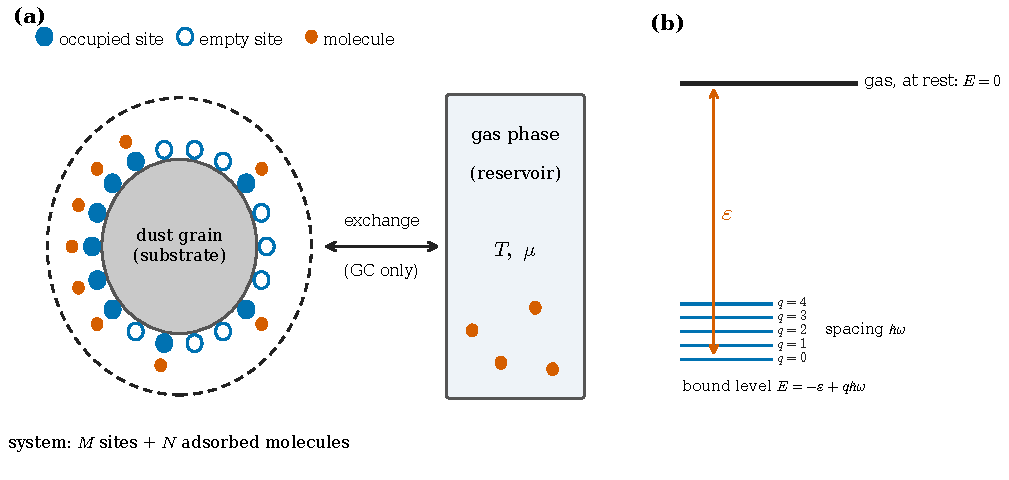
\includegraphics[width=\textwidth]{figures/fig_model.pdf}
\caption{(a) The system (dashed line) consists of the $M$ adsorption sites of one grain and the $N$ molecules adsorbed on them; the surrounding gas is a reservoir at temperature $T$ and chemical potential $\mu$ that enters only in the grand-canonical ensemble. (b) Energy levels of one site in Model~B: gas-phase molecule at rest ($E=0$), and the ladder of bound levels $E=-\eps+q\hw$ ($\eps=20\hw$ in the numerics). An empty site has $E=0$.}
\label{fig:model}
\end{figure}

\begin{figure}[tbp]
\centering
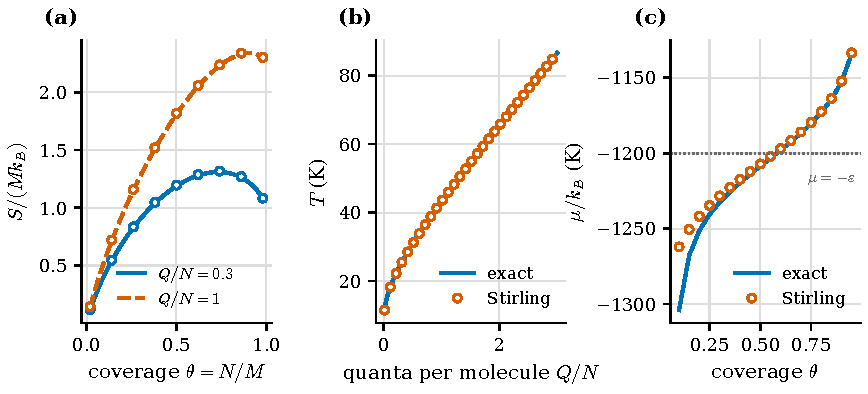
\includegraphics[width=\textwidth]{figures/fig_micro.pdf}
\caption{Microcanonical quantities for $M=1000$, $g=3$, $\eps=20\,\hw$, $\hw/\kB=\SI{60}{K}$. Lines (``exact): $\kB\ln\Omega$ with central finite differences; open markers: Stirling formulas \cref{eq:Sstirling,eq:Tmicro,eq:mumicro}. (a) Entropy per site against coverage for $Q/N=0.3$ and $1$. (b) $T$ against $Q/N$ at $N=300$. (c) $\mu/\kB$ against coverage for $Q/N=0.3$; the dotted line is $\mu=-\eps$, crossed where $\theta=\zv/(1+\zv)$.}
\label{fig:micro}
\end{figure}

% ===================================================== 5 CANONICAL
\section{Canonical ensemble}
\label{sec:can}

At fixed $(M,N,T)$ the system exchanges only energy with a heat bath. The partition function is the sum of $\ee^{-\beta E}$ over all microstates with $N$ adsorbed molecules. The configurational choice of sites contributes the factor $\binom{M}{N}$ and the binding energy the factor $\ee^{\beta N\eps}$. The vibrational sum factorises over the $G=gN$ independent oscillators, each contributing $\sum_{q\ge0}\ee^{-\beta\hw q}=(1-\ee^{-\beta\hw})^{-1}$:
\begin{equation}
 \boxed{\;Z_N=\binomc{M}{N}\,\ee^{\beta N\eps}\,\zv^{N},\qquad \zv=\bigl(1-\ee^{-\beta\hw}\bigr)^{-g}\;}
 \label{eq:Z}
\end{equation}
(checked against explicit sums over all enumerated microstates, test V3a). Equivalent to summing the multiplicity over $Q$: $Z_N=\sum_{Q}\Omega\,\ee^{-\beta E}$. The Helmholtz free energy is $F=-\kB T\ln Z_N$, explicitly
\begin{equation}
 F=-\kB T\Bigl[\ln\binomc{M}{N}+\beta N\eps+N\ln\zv\Bigr].
\end{equation}

\paragraph{Average energy.}
\begin{equation}
 \ave{E}=-\frac{\partial\ln Z_N}{\partial\beta}=-N\eps+\frac{gN\hw}{\ee^{\beta\hw}-1}=-N\eps+gN\hw\,\nbar,
 \label{eq:Ecan}
\end{equation}
using $\partial\ln\zv/\partial\beta=-g\hw/(\ee^{\beta\hw}-1)$. At the temperature \cref{eq:Tmicro} this equals the microcanonical energy; \cref{eq:Ecan} is identical to \cref{eq:caloric}. The binomial factor does not contribute, because $\binom{M}{N}$ does not depend on $\beta$ (the energy is blind to \emph{which} sites are occupied).

\paragraph{Fluctuations.} The quanta are distributed as a negative binomial law, $P(Q)\propto\binom{Q+G-1}{Q}\ee^{-\beta\hw Q}$, with
\begin{equation}
 \Var E=\hw^{2}\Var Q=gN\hw^{2}\frac{\ee^{x}}{(\ee^{x}-1)^{2}}=\kB T^{2}C_N,\qquad
 \frac{\sigma_Q}{\ave{Q}}=\sqrt{\frac1G+\frac1Q}.
 \label{eq:varEcan}
\end{equation}
(Both moments were confirmed by summing the exact distribution, test V7b.) The relative width decays as $N^{-1/2}$.

\paragraph{Entropy and chemical potential.} $S_{\rm can}=\kB(\ln Z_N+\beta\ave{E})$. The thermodynamic chemical potential obtained from the canonical free energy, $\mu=(\partial F/\partial N)_{T,M}$ with $\dd\ln\binom{M}{N}/\dd N=\ln[(M-N)/N]$, is
\begin{equation}
 \mu=-\eps-\kB T\ln\zv+\kB T\ln\frac{N}{M-N},
\end{equation}
identical to \cref{eq:mumicro}: the canonical ensemble reproduces the microcanonical chemical potential at the same $T$.

\begin{figure}[tbp]
\centering
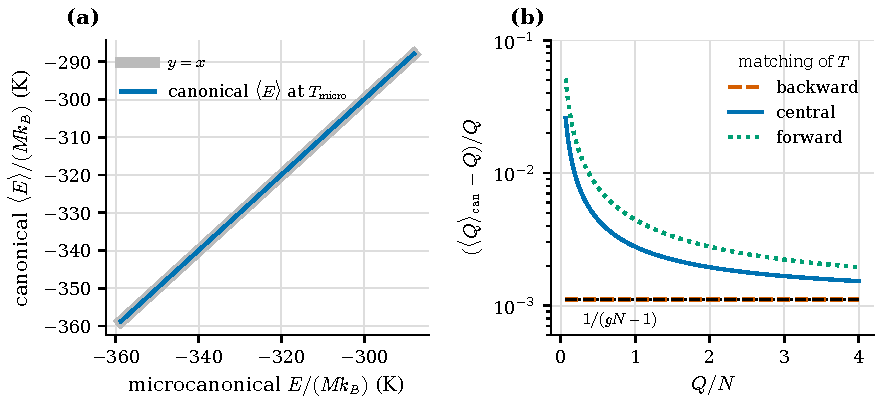
\includegraphics[width=\textwidth]{figures/fig_canonical.pdf}
\caption{Canonical check for $M=1000$, $N=300$, $g=3$, $\eps=20\,\hw$. The canonical ensemble is evaluated at the temperature obtained from the \emph{exact} $\ln\Omega$. (a) Canonical $\ave{E}/(M\kB)$ against microcanonical $E/(M\kB)$ (thick grey line: $y=x$). (b) Relative difference of the vibrational part, $(\ave{Q}-Q)/Q$, for backward, central and forward finite-difference temperatures; the dash-dotted line is the exact backward result $1/(gN-1)$, \cref{eq:propQ}.}
\label{fig:can}
\end{figure}

% ================================================= 6 GRAND CANONICAL
\section{Grand-canonical ensemble}
\label{sec:gc}

At fixed $(M,T,\mu)$ the system exchanges energy and molecules with the gas reservoir. Summing the canonical results over $N$,
\begin{equation}
 \Xi=\sum_{N=0}^{M}\ee^{\beta\mu N}Z_N=\sum_{N=0}^{M}\binomc{M}{N}\lambda^{N}
 =\boxed{\;(1+\lambda)^{M},\qquad \lambda=\ee^{\beta(\mu+\eps)}\zv\;}
 \label{eq:Xi}
\end{equation}
by the binomial theorem; equivalently $\Xi$ is the $M$-th power of the single-site factor $1+\ee^{\beta(\mu+\eps)}\zv$, because sites are independent. The grand potential is $\Phi=-\kB T\ln\Xi=-M\kB T\ln(1+\lambda)$.

\paragraph{Average occupancy (Langmuir isotherm).}
\begin{equation}
 \boxed{\;\ave{N}=\kB T\frac{\partial\ln\Xi}{\partial\mu}=\frac{M\lambda}{1+\lambda},\qquad
 \theta=\frac{1}{1+\ee^{-\beta(\mu+\eps)}\,\zv^{-1}}\;}
 \label{eq:Langmuir}
\end{equation}
This has the form of the Langmuir isotherm \citep{langmuir1918}, here with a vibrational factor $\zv$. It reproduces \cref{eq:mumicro}, $\theta/(1-\theta)=\lambda$: with $(T,\mu)$ taken from the microcanonical ensemble the grand-canonical occupancy equals $N$.

\paragraph{Fluctuations.} $P(N)=\binom{M}{N}\lambda^N/(1+\lambda)^M$ is binomial, and
\begin{equation}
 \Var N=\kB T\frac{\partial\ave N}{\partial\mu}=M\theta(1-\theta),\qquad
 \frac{\sigma_N}{\ave N}=\sqrt{\frac{1-\theta}{M\theta}} .
 \label{eq:varN}
\end{equation}
\paragraph{Energy.} Differentiating $\ln\Xi$ at fixed $\beta\mu$,
\begin{equation}
 \ave{E}=\ave{N}\bigl(-\eps+g\hw\,\nbar\bigr),\qquad
 \Var E=M\Bigl[\theta(1-\theta)u^{2}+\theta\,\sigma_h^{2}\Bigr],
 \label{eq:EGC}
\end{equation}
where $u=-\eps+g\hw\nbar$ and $\sigma_h^{2}=g\hw^{2}\ee^{x}/(\ee^{x}-1)^{2}$ is the variance of the vibrational energy of one adsorbed molecule, and $\Cov(E,N)=M\theta(1-\theta)u$. The determinant of the covariance matrix is
\begin{equation}
 \det\Cov(E,N)=M^{2}\theta^{2}(1-\theta)\,\sigma_h^{2}>0,
 \label{eq:detcov}
\end{equation}
which is strictly positive for $0<\theta<1$ and finite $T$ (and, in contrast to Model~A, nonzero because of the vibrations). \Cref{eq:varN,eq:EGC,eq:detcov} were validated by exact summation and by numerical Hessians of $\ln\Xi$ (tests V6, V7a).

\paragraph{Relation to the gas phase.} In equilibrium $\mu$ equals the chemical potential of the gas. For a dilute gas of structureless molecules of mass $m$ at number density $n$, $\mu_{\rm gas}=\kB T\ln(n\Lambda^{3})$ with $\Lambda=h/\sqrt{2\pi m\kB T}$. Then $\lambda=n\Lambda^{3}\ee^{\eps/\kB T}\zv$ and
\begin{equation}
 \theta=\frac{n}{n+n_{*}(T)},\qquad n_{*}(T)=\Lambda^{-3}\,\ee^{-\eps/\kB T}\,\zv^{-1}.
 \label{eq:isotherm_n}
\end{equation}
The ideal gas thus appears only as a source of $\mu$; the adsorbed layer itself is a lattice.

\begin{figure}[tbp]
\centering
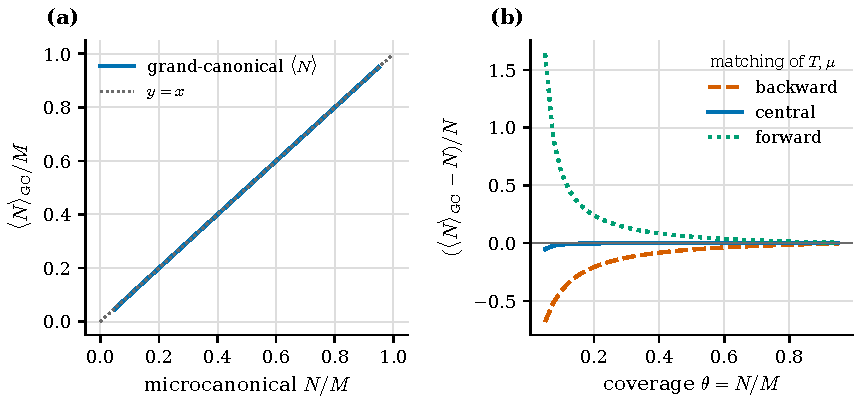
\includegraphics[width=\textwidth]{figures/fig_grand.pdf}
\caption{Grand-canonical check for $M=10^{4}$, $g=3$, $\eps=20\,\hw$, $Q/N=0.3$. (a) $\ave{N}_{\rm GC}/M$ evaluated at the microcanonical $(T,\mu)$ (central differences) against $N/M$. (b) Relative difference $(\ave{N}_{\rm GC}-N)/N$ for backward, central and forward definitions; backward and forward results bracket the microcanonical value, as in the exact Model~A relation \cref{eq:bracketA}.}
\label{fig:grand}
\end{figure}

% ====================================================== 7 COMPARISON
\section{Comparison of the three ensembles}
\label{sec:compare}

\subsection{Protocol}
\begin{enumerate}
\item Choose a microcanonical state $(M,N,Q)$, i.e.\ $E=-N\eps+Q\hw$.
\item Obtain $T$ and $\mu$ from $\Omega$: analytically at large $N$ (\cref{eq:Tmicro,eq:mumicro}) or from the exact finite differences \cref{eq:fd}.
\item Canonical ensemble at $(M,N,T)$: compute $\ave{E}$ from \cref{eq:Ecan} and compare with $E$.
\item Grand-canonical ensemble at $(M,T,\mu)$: compute $\ave{N}$ from \cref{eq:Langmuir} and compare with $N$.
\end{enumerate}

\subsection{Leading-order equivalence (analytic)}
With $T$ and $\mu$ defined through the Stirling entropy, \cref{eq:Tmicro,eq:Ecan} and \cref{eq:mumicro,eq:Langmuir} give $\ave{E}_{\rm can}=E$ and $\ave{N}_{\rm GC}=N$ \emph{identically}, and also $\ave{E}_{\rm GC}=E$ and $\ave{Q}_{\rm GC}=Q$ (\cref{eq:EGC}). This is the Legendre-transform structure of the ensembles: the saddle-point of the sum over the exact distribution sits at the microcanonical state. It verifies the algebra, but the equality holds because the Stirling entropy was used to \emph{define} $T$ and $\mu$; it is not yet a statement about the exact finite model. The next subsections test the equivalence against the exact $\ln\Omega$.

\subsection{Exact finite-system result: agreement is not exact}
\label{sec:exactfinite}

\begin{proposition}[canonical energy at exact finite-difference temperature]\label{prop:Q}
With $T$ defined by the backward or forward difference \cref{eq:fd}, $G=gN$,
\begin{equation}
 \ave{Q}_{\rm can}^{\rm bwd}=\frac{G}{G-1}\,Q,\qquad
 \ave{Q}_{\rm can}^{\rm fwd}=\frac{G}{G-1}(Q+1).
 \label{eq:propQ}
\end{equation}
\end{proposition}
\begin{proof}
For the vibrational factor $\Omega_{\rm v}(Q)=\binom{Q+G-1}{Q}$, $\Omega_{\rm v}(Q)/\Omega_{\rm v}(Q-1)=(Q+G-1)/Q$ and $\Omega_{\rm v}(Q+1)/\Omega_{\rm v}(Q)=(Q+G)/(Q+1)$ (the configurational factor does not depend on $Q$). Hence $\ee^{\beta\hw}-1=(G-1)/Q$ (backward) or $(G-1)/(Q+1)$ (forward), and \cref{eq:Ecan} gives $\ave{Q}=G/(\ee^{\beta\hw}-1)$.
\end{proof}
The relative errors are $1/(G-1)$ and $(Q+G)/[Q(G-1)]$ respectively; the central choice lies between them. They are never zero. The reason is that the canonical mean $\ave{Q}$ is a mean over a distribution of width $\sigma_Q\propto\sqrt{N}$ whose maximum, not whose mean, is located by the logarithmic slope of $\Omega$, and the two differ by $O(1)$ for the skewed negative-binomial law. The \emph{only} definition giving exact equality is the Stirling one, $\ee^{\beta\hw}=1+G/Q$, which is not the slope of the exact multiplicity.

For the chemical potential in Model~B the discrete derivative at fixed $E$ moves $Q$ by $r$ quanta and no closed form is available, so the grand-canonical mismatch was computed exactly by numerical evaluation. For Model~A the exact result is \cref{eq:bracketA}. \Cref{tab:compare} compares all three ensembles for the representative state, and \cref{tab:finite} shows the dependence on $M$.

\begin{table}[tbp]
\centering
\caption{Comparison of the three ensembles for the representative state ($M=10^{6}$, $N=3\times10^{5}$, $Q=9\times10^{4}$, $g=3$, $\eps=20\hw$, $\hw/\kB=\SI{60}{K}$). Canonical and grand-canonical entries are evaluated at the microcanonical $T$ and $\mu$ from \emph{exact central finite differences}, \cref{eq:fd}. The last two columns give the relative difference from the microcanonical value. $E/(M\kB)$ is in kelvin, entropies per site in units of $\kB$; the canonical $N$ is fixed by definition.}
\label{tab:compare}
\footnotesize
\setlength{\tabcolsep}{4pt}
\begin{tabular}{@{}l r r r r r@{}}
\toprule
Quantity & micro & canonical & grand-can. & rel.\ diff.\ (can.) & rel.\ diff.\ (GC) \\
\midrule
$N$ (adsorbed molecules) & 300000.0 & 300000.0 & 300000.5 & $0$ & $+1.7\!\times\!10^{-6}$ \\
$Q$ (vibrational quanta) & 90000.0 & 90000.6 & 90000.8 & $+6.7\!\times\!10^{-6}$ & $+8.4\!\times\!10^{-6}$ \\
$E/(Mk_B)$ (K) & $-$354.60000 & $-$354.59996 & $-$354.60057 & $-1.0\!\times\!10^{-7}$ & $+1.6\!\times\!10^{-6}$ \\
$S/(Mk_B)$ & 0.912440 & 0.912448 & 0.912456 & $+8.9\!\times\!10^{-6}$ & $+1.8\!\times\!10^{-5}$ \\
\bottomrule
\end{tabular}

\end{table}

\begin{table}[tbp]
\centering
\caption{Finite-size dependence of the relative deviations $(\ave{Q}_{\rm can}-Q)/Q$ and $(\ave{N}_{\rm GC}-N)/N$ for $\theta=0.30$, $Q/N=0.30$ and the three finite-difference conventions. All columns decrease as $1/M$ once $M$ is large; for $M=10^{3}$ the central $\mu$ differs by about $\num{\numdevNkilo}$ in relative occupancy because removing one molecule at fixed $E$ requires $r=20$ quanta of the $Q=90$ available.}
\label{tab:finite}
\footnotesize
\setlength{\tabcolsep}{3.4pt}
\begin{tabular}{@{}c ccc ccc@{}}
\toprule
 & \multicolumn{3}{c}{$(\ave{Q}_{\rm can}-Q)/Q$} & \multicolumn{3}{c}{$(\ave{N}_{\rm GC}-N)/N$}\\
\cmidrule(lr){2-4}\cmidrule(lr){5-7}
$M$ & bwd & central & fwd & bwd & central & fwd\\
\midrule
$10^{3}$ & $+1.1\!\times\!10^{-3}$ & $+6.7\!\times\!10^{-3}$ & $+1.2\!\times\!10^{-2}$ & $-8.2\!\times\!10^{-1}$ & $-1.1\!\times\!10^{-1}$ & $+1.3\!\times\!10^{0}$ \\
$10^{4}$ & $+1.1\!\times\!10^{-4}$ & $+6.7\!\times\!10^{-4}$ & $+1.2\!\times\!10^{-3}$ & $-1.3\!\times\!10^{-1}$ & $-9.5\!\times\!10^{-4}$ & $+1.3\!\times\!10^{-1}$ \\
$10^{5}$ & $+1.1\!\times\!10^{-5}$ & $+6.7\!\times\!10^{-5}$ & $+1.2\!\times\!10^{-4}$ & $-1.3\!\times\!10^{-2}$ & $+7.0\!\times\!10^{-6}$ & $+1.3\!\times\!10^{-2}$ \\
$10^{6}$ & $+1.1\!\times\!10^{-6}$ & $+6.7\!\times\!10^{-6}$ & $+1.2\!\times\!10^{-5}$ & $-1.3\!\times\!10^{-3}$ & $+1.7\!\times\!10^{-6}$ & $+1.3\!\times\!10^{-3}$ \\
$10^{7}$ & $+1.1\!\times\!10^{-7}$ & $+6.7\!\times\!10^{-7}$ & $+1.2\!\times\!10^{-6}$ & $-1.3\!\times\!10^{-4}$ & $+1.8\!\times\!10^{-7}$ & $+1.3\!\times\!10^{-4}$ \\
\bottomrule
\end{tabular}

\end{table}

\subsection{Finite-size scaling and the thermodynamic limit}
\label{sec:tdl}

\Cref{fig:scaling}(a,b) shows $|\ave{Q}_{\rm can}/Q-1|$ and $|\ave{N}_{\rm GC}/N-1|$ against $M$ from $M=400$ to about $4\times10^{8}$. Each convention converges as $M^{-1}$ (fits of the central-scheme curves over the six largest $M$ give slopes $\num{\numslopeQ}$ and $\num{\numslopeN}$; test V9). The forward and backward $\mu$ errors are large for moderate $M$ (about $\pm1.3\times10^{3}/M$, i.e.\ roughly $3r^{2}/M$ for these parameters) because a one-molecule step at fixed $E$ moves $Q$ by $r=20$ quanta; the central scheme cancels the leading error, so its curve shows a crossover (and a sign change) before settling onto its asymptotic $1/M$ law with a much smaller coefficient. Practically: the microcanonical $\mu$ is a well-defined derivative only when $Q\gg r^{2}=\num{\numrsq}$, i.e.\ for $M$ of order $10^{4}$ or larger in this example.

The deeper reason for equivalence in the limit $M\to\infty$ is convexity. The entropy per site $s(e,\theta)=\lim S/(M\kB)$ is the Legendre--Fenchel transform of $\varphi(\beta,\beta\mu)=\ln\Xi/M=\ln(1+\lambda)$, which is analytic. Its Hessian is the covariance matrix per site, with determinant $\theta^{2}(1-\theta)\sigma_h^{2}>0$ \cref{eq:detcov}, so $\varphi$ is strictly convex and $s$ is strictly concave; the standard criterion \citep{touchette2015} then guarantees ensemble equivalence at the thermodynamic, macrostate and measure levels. In Model~A the determinant vanishes, $\varphi$ is only convex along one direction, and the Legendre map from $(\beta,\beta\mu)$ to $(e,\theta)$ is many-to-one: this is the formal origin of the degeneracy found in \cref{sec:modelA}.

\begin{figure}[tbp]
\centering
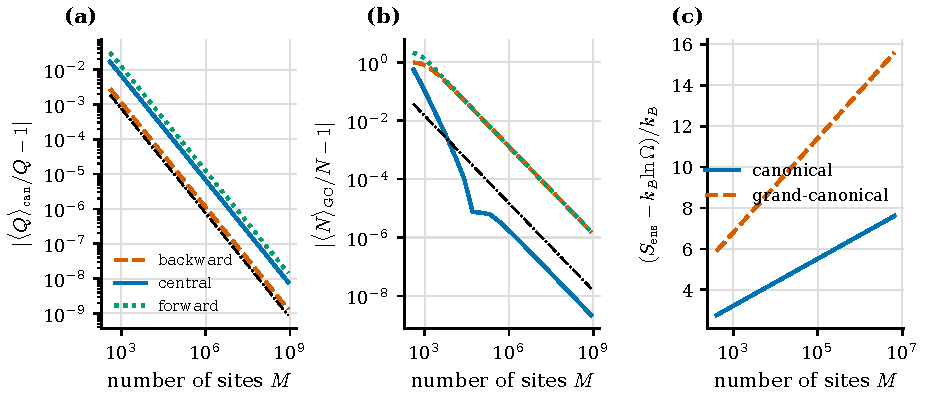
\includegraphics[width=\textwidth]{figures/fig_scaling.pdf}
\caption{Finite-size scaling at $\theta=0.30$, $Q/N=0.30$, $g=3$, $\eps=20\hw$ ($M=400$ to $4\times10^{8}$). (a) $|\ave{Q}_{\rm can}/Q-1|$ and (b) $|\ave{N}_{\rm GC}/N-1|$ for the three finite-difference conventions; the black dash-dotted line is a $\propto1/M$ guide. (c) Entropy offsets $[S_{\rm ens}-\kB\ln\Omega]/\kB$ for the canonical and grand-canonical ensembles at the Stirling-matched parameters; they grow only logarithmically, so entropy \emph{per site} converges.}
\label{fig:scaling}
\end{figure}

\subsection{Entropy}
\label{sec:entropy}

Replacing the sum over $Q$ in $Z_N$ by a Gaussian of variance $\sigma_Q^{2}=gN\ee^{x}/(\ee^{x}-1)^{2}$ about its maximum on the integer lattice gives
\begin{equation}
 \frac{S_{\rm can}-\kB\ln\Omega}{\kB}=\tfrac12\ln\bigl(2\pi\sigma_Q^{2}\bigr)+O(N^{-1}),
 \label{eq:Scan}
\end{equation}
and the corresponding two-dimensional Gaussian sum over $(N,Q)$ in $\Xi$ gives
\begin{equation}
 \frac{S_{\rm GC}-\kB\ln\Omega}{\kB}=\ln 2\pi+\tfrac12\ln\det\Cov(N,Q)+O(M^{-1}),\qquad
 \det\Cov(N,Q)=M^{2}\theta^{2}(1-\theta)\,\sigma_h^{2}/\hw^{2}.
 \label{eq:SGC}
\end{equation}
Here $S_{\rm ens}=\kB(\ln Z+\beta\ave{E})$ or $\kB(\ln\Xi+\beta\ave{E}-\beta\mu\ave{N})$ is evaluated at the Stirling-matched parameters, for which $\ave{Q}=Q$ and $\ave{N}=N$ exactly. Both formulas were verified numerically at $M=10^{6}$ (agreement to $10^{-6}$, test V8), and \cref{fig:scaling}(c) shows the logarithmic growth: the canonical offset increases from $\num{\numentCanSmall}$ at $M=400$ to $\num{\numentCanLarge}$ at $M\approx6.6\times10^{6}$, the grand-canonical one reaches $\num{\numentGCLarge}$. Because $\ln M/M\to0$, all entropies per site coincide in the limit; at $M=10^{6}$ the three values in \cref{tab:compare} agree to $2\times10^{-5}$.

\subsection{Fluctuations}
The microcanonical ensemble has no fluctuations of $E$ or $N$ by construction. In the canonical ensemble $E$ fluctuates with relative vibrational width \cref{eq:varEcan}, and in the grand-canonical ensemble $N$ fluctuates with the binomial width \cref{eq:varN}; for the representative state $\sigma_N/\ave N=\num{\numrelfluctN}$. Both decay as $M^{-1/2}$ (\cref{fig:fluct}), the usual statement that the ensembles differ only in how much of the (vanishingly narrow) distribution they retain. For $M$ of order $10^6$ these fluctuations are of order $10^{-3}$, which is why the equilibrium occupancy is a sharp function of the control parameters for a typical grain.

\begin{figure}[tbp]
\centering
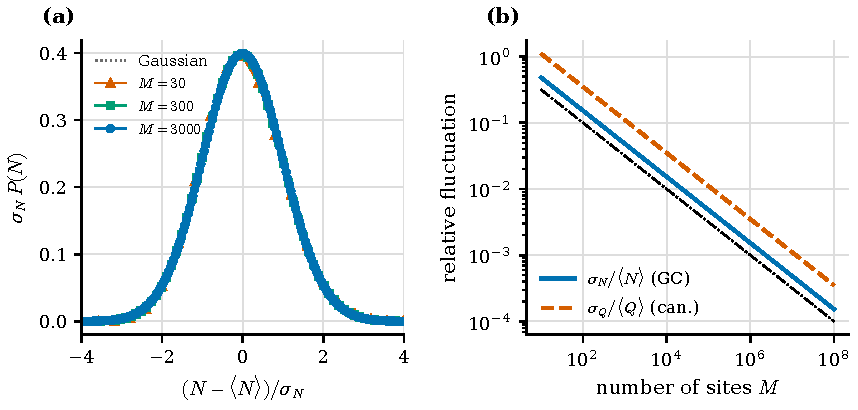
\includegraphics[width=\textwidth]{figures/fig_fluct.pdf}
\caption{Fluctuations. (a) Exact binomial grand-canonical distribution $P(N)$ rescaled by its standard deviation for $\theta=0.3$ and $M=30$, $300$, $3000$, compared with the standard Gaussian (grey dotted). (b) Relative fluctuations of $N$ (grand-canonical) and of the vibrational quanta $Q$ (canonical, $Q/N=0.3$) against $M$; the black dash-dotted line is a $\propto M^{-1/2}$ guide.}
\label{fig:fluct}
\end{figure}

% ================================================ 8 NUMERICAL VALIDATION
\section{Numerical validation}
\label{sec:validation}

Every closed-form result above is checked independently by the program \texttt{code/validate.py}, whose \num{\numnchecks} tests all pass (\cref{app:valid}). The checks are of four kinds.
\begin{enumerate}
\item \textbf{Brute-force enumeration.} All $2^{14}$ occupation patterns of Model~A; and \emph{all} microstates of Model~B (explicit occupation \emph{and} explicit quantum numbers of every mode) for $(M,g)=(4,1)$, $(3,2)$ and $(3,3)$. The enumerated multiplicities equal \cref{eq:Omega} exactly; the brute-force sums for $Z_N$, $\Xi$ and $P(N)$ agree with \cref{eq:Z,eq:Xi} to better than $10^{-9}$ (test~V3; residuals are consistent with the truncation of the vibrational sum).
\item \textbf{Derivatives.} The analytic $T$ and $\mu$ of \cref{eq:Tmicro,eq:mumicro} equal the numerical derivatives of the Stirling entropy to $2\times10^{-8}$, which tests the signs and the $\partial Q/\partial N=r$ term.
\item \textbf{Exact identities.} \Cref{eq:propQ}, \cref{eq:bracketA}, the covariance entries and determinants, the normalisation and moments of the exact $P(N)$ and $P(Q)$.
\item \textbf{Asymptotics.} The entropy offsets \cref{eq:Scan,eq:SGC} and the $1/M$ scaling (\cref{fig:scaling}).
\end{enumerate}
The finite differences of $\ln\Omega$ are computed as exact sums of logarithms of integers rather than as differences of $\ln\Gamma$ values, which avoids cancellation up to $M\sim10^{9}$ (double precision).

% ================================================== 9 ASTROPHYSICAL USE
\section{Illustration: equilibrium coverage as a function of temperature and gas density}
\label{sec:astro}

Combining \cref{eq:isotherm_n} with the illustrative parameters ($\eps/\kB=\SI{1200}{K}$, $\hw/\kB=\SI{60}{K}$, $g=3$, $m=28\,\mathrm{u}$, structureless gas molecules), \cref{fig:astro}(a) shows the equilibrium coverage as a function of temperature for three gas densities. The coverage falls from nearly one to nearly zero over a few kelvin around \SIrange{20}{30}{K}: the grain surface is in a Langmuir-type ``condensed--evaporated'' crossover that moves to higher temperature as $n$ increases. For the representative state of \cref{sec:micro}, $\mu/\kB=\SI{\nummuKstir}{K}$ at $T=\SI{\numTstir}{K}$ corresponds to $n=\ee^{\beta\mu}\Lambda^{-3}\approx\SI{\numngas}{cm^{-3}}$ with $\Lambda=\numlamT\,\text{\AA}$. These numbers illustrate how $\mu$ and $T$ are related to gas conditions; they are not predictions for any real species.

Equilibrium requires that desorption be fast. With the first-order estimate $t_{\rm des}=\nu_0^{-1}\ee^{\eps/\kB T}$ and an attempt frequency $\nu_0=10^{12}\,\mathrm{s^{-1}}$ \citep[order of magnitude, cf.][]{hasegawa1992}, \cref{fig:astro}(b) gives $t_{\rm des}\approx\SI{\numtdesRep}{yr}$ at $T=\SI{\numTstir}{K}$, but $t_{\rm des}$ exceeds $10^{10}$\,yr below about \SI{\numTdesTenGyr}{K} and exceeds one year below about \SI{\numTdesOneYr}{K} for this binding energy. At lower temperatures a surface that starts empty cannot relax to the equilibrium isotherm by thermal desorption alone, and the occupancy is controlled by kinetics (adsorption from the gas, non-thermal desorption, surface reactions), which is the domain of rate-equation models \citep{hasegawa1992,cuppen2017}. The equilibrium ensembles are therefore a reference state and a consistency check, not a substitute for those models.

\begin{figure}[tbp]
\centering
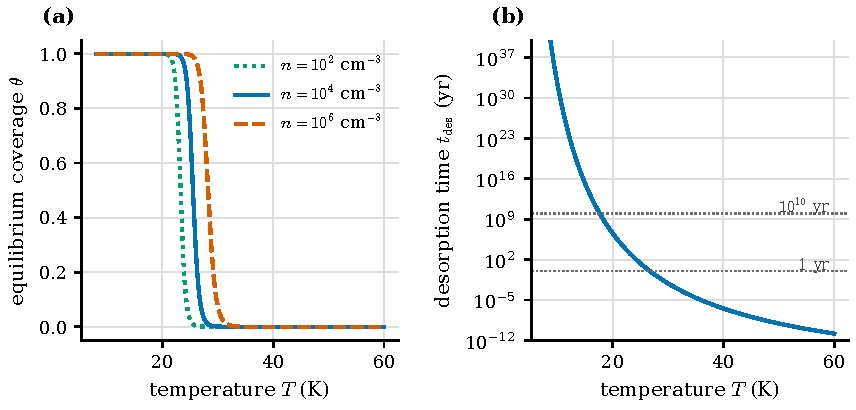
\includegraphics[width=\textwidth]{figures/fig_astro.pdf}
\caption{Illustrative equilibrium adsorption, with $\eps/\kB=\SI{1200}{K}$, $\hw/\kB=\SI{60}{K}$, $g=3$ and $m=28\,\mathrm{u}$ (parameters not fitted to any species). (a) Equilibrium coverage from \cref{eq:isotherm_n} against temperature for gas densities $n=10^{2}$, $10^{4}$ and $10^{6}\,\mathrm{cm^{-3}}$. (b) Thermal desorption time $t_{\rm des}=\nu_0^{-1}\ee^{\eps/\kB T}$ with $\nu_0=10^{12}\,\mathrm{s^{-1}}$; dotted lines mark $1$\,yr and $10^{10}$\,yr.}
\label{fig:astro}
\end{figure}

% ======================================================== 10 LIMITATIONS
\section{Limitations and possible extensions}
\label{sec:limits}

\begin{itemize}
\item \textbf{Equilibrium versus kinetics.} Real grain surfaces in cold regions are generally not in adsorption--desorption equilibrium (see above); this study provides the equilibrium reference only.
\item \textbf{Independent sites.} Lateral interactions are neglected. Nearest-neighbour interactions would turn the model into an interacting lattice gas with collective behaviour (for example condensation-like transitions) and a non-trivial concavity analysis; this is not attempted.
\item \textbf{Identical sites.} Amorphous substrates have a distribution of binding energies. For independent sites with a distribution of $\eps$ the grand-canonical occupancy would be an average of \cref{eq:Langmuir} over that distribution; fixed-$N$ ensembles would then have to sum over site classes. Not implemented.
\item \textbf{Single layer, single species, structureless molecule.} No multilayers, mixtures, rotations or electronic structure; only $g$ identical harmonic modes (no anharmonicity or mode-dependent frequencies).
\item \textbf{Illustrative parameters.} $\eps$, $\hw$, $g$, $m$ are order-of-magnitude choices. Binding energies depend strongly on the species and on the substrate, and compilations are given by \citet{cuppen2017}.
\item \textbf{Finite-difference definition of $T$ and $\mu$.} For an isolated finite system the microcanonical $T$ and $\mu$ are not unique (\cref{sec:fd}); the quoted finite-size differences depend on that convention, whereas the thermodynamic-limit equivalence does not.
\item \textbf{Substrate not counted.} The heat capacity of the grain itself is outside the system; stochastic effects for very small grains are not addressed.
\end{itemize}

% ======================================================== 11 CONCLUSIONS
\section{Conclusions}
\label{sec:conclusions}

The three ensembles were constructed from first principles for a lattice of $M$ independent adsorption sites. The bare binary model (Model~A) is exactly solvable, but because $E=-N\eps$ it fixes only $(\mu+\eps)/T$ and makes the canonical energy test empty; giving each adsorbed molecule $g$ harmonic modes (Model~B) removes this degeneracy. For Model~B, $\Omega=\binom{M}{N}\binom{Q+gN-1}{Q}$, $\ee^{\beta\hw}=1+gN/Q$, $\mu=-\eps-\kB T\ln\zv+\kB T\ln[N/(M-N)]$; the canonical energy is $\ave E=-N\eps+gN\hw\nbar$ and the grand-canonical occupancy is the Langmuir form $\ave N=M\lambda/(1+\lambda)$ with $\lambda=\ee^{\beta(\mu+\eps)}\zv$.

At leading order the three descriptions are identical. For the finite system \emph{exact agreement is not possible}: with $T$ and $\mu$ defined from the exact multiplicity the canonical and grand-canonical averages differ from the microcanonical values by relative amounts of order $1/N$ (closed forms \cref{eq:propQ,eq:bracketA}; numerical $M^{-1}$ scaling over six decades), and entropies differ by $O(\ln M)$ Gaussian terms. Agreement holds in the thermodynamic limit because the entropy density is strictly concave. For a grain with about $10^{6}$ sites the relative differences are of order $10^{-6}$, whereas for $10^{3}$ sites they can reach about $10\%$ in the chemical-potential matching. The astrophysical relevance is as an equilibrium reference for grain-surface occupancy; the stated limitations, above all the neglect of kinetics and of site interactions and heterogeneity, apply.

% ============================================================ REFERENCES
\bibliographystyle{unsrtnat}
\bibliography{references}

% ============================================================ APPENDICES
\appendix
\section{Validation tests}
\label{app:valid}

\Cref{tab:valid} lists every automated test (\texttt{code/validate.py}). The deviation is the maximum absolute or relative difference between the quantity computed from the closed form in this report and the independent numerical evaluation; ``0'' denotes exact integer agreement.

{\small
\begin{longtable}{@{}l p{9.4cm} r l@{}}
\caption{Automated verification of the analytic results.}\label{tab:valid}\\
\toprule
ID & Test & deviation & status\\
\midrule
\endfirsthead
\toprule
ID & Test & deviation & status\\
\midrule
\endhead
\bottomrule
\endfoot
V1 & Model A: all $2^M$ occupation patterns counted vs.\ $\binom{M}{N}$ & $0$ & pass \\
V2 & Model B: enumerated $\Omega(N,Q)$ vs.\ $\binom{M}{N}\binom{Q+gN-1}{Q}$ [$M=4,\ g=1,\ Q\leq 30$] & $0$ & pass \\
V3a & Canonical $Z_N$: brute-force sum vs.\ $\binom{M}{N}e^{\beta N\varepsilon}z_v^{N}$ [$M=4,\ g=1$] & $1.2\times10^{-14}$ & pass \\
V3b & Grand $\Xi=(1+\lambda)^M$ and $P(N)$: brute-force sum vs.\ closed form [$M=4,\ g=1$] & $3.1\times10^{-15}$ & pass \\
V2 & Model B: enumerated $\Omega(N,Q)$ vs.\ $\binom{M}{N}\binom{Q+gN-1}{Q}$ [$M=3,\ g=2,\ Q\leq 14$] & $0$ & pass \\
V3a & Canonical $Z_N$: brute-force sum vs.\ $\binom{M}{N}e^{\beta N\varepsilon}z_v^{N}$ [$M=3,\ g=2$] & $1.2\times10^{-14}$ & pass \\
V3b & Grand $\Xi=(1+\lambda)^M$ and $P(N)$: brute-force sum vs.\ closed form [$M=3,\ g=2$] & $1.0\times10^{-15}$ & pass \\
V2 & Model B: enumerated $\Omega(N,Q)$ vs.\ $\binom{M}{N}\binom{Q+gN-1}{Q}$ [$M=3,\ g=3,\ Q\leq 8$] & $0$ & pass \\
V3a & Canonical $Z_N$: brute-force sum vs.\ $\binom{M}{N}e^{\beta N\varepsilon}z_v^{N}$ [$M=3,\ g=3$] & $2.8\times10^{-10}$ & pass \\
V3b & Grand $\Xi=(1+\lambda)^M$ and $P(N)$: brute-force sum vs.\ closed form [$M=3,\ g=3$] & $2.8\times10^{-10}$ & pass \\
V4a & Stirling: $1/k_BT=\partial S/\partial E|_N$, analytic vs.\ numerical derivative & $1.7\times10^{-8}$ & pass \\
V4b & Stirling: $-\mu/k_BT=\partial S/\partial N|_E$, analytic vs.\ numerical derivative & $1.7\times10^{-9}$ & pass \\
V5a & Canonical $\langle Q\rangle$ at backward-difference $T$ equals $QG/(G-1)$, $G=gN$ & $4.4\times10^{-16}$ & pass \\
V5b & Canonical $\langle Q\rangle$ at forward-difference $T$ equals $G(Q+1)/(G-1)$ & $4.4\times10^{-16}$ & pass \\
V5c & Model A: $\langle N\rangle_{\rm GC}=MN/(M+1)$ (backward), $M(N+1)/(M+1)$ (forward) & $2.2\times10^{-16}$ & pass \\
V5d & Model B: $\langle N\rangle^{\rm back}_{\rm GC}<N<\langle N\rangle^{\rm fwd}_{\rm GC}$, $M=400$--$10^5$ (0 = holds) & $0$ & pass \\
V6a & Model B: $\mathrm{Cov}(E,N)$, numerical Hessian of $\ln\Xi$ vs.\ closed form & $2.1\times10^{-7}$ & pass \\
V6e & Model B: $\det\mathrm{Cov}=M^2\theta^2(1-\theta)\sigma_h^2$ (algebraic identity) & $2.6\times10^{-13}$ & pass \\
V6b & Model B: $\mathrm{Var}(N)$ numerical vs.\ $M\theta(1-\theta)$ & $3.3\times10^{-8}$ & pass \\
V6c & Model B: $\mathrm{Var}(E)$ numerical vs.\ closed form & $1.1\times10^{-7}$ & pass \\
V6d & Model A: $\det\mathrm{Cov}(E,N)=0$ (relative to $\mathrm{Var}E\,\mathrm{Var}N$) & $0$ & pass \\
V7a & Grand: normalisation, $\langle N\rangle$, $\mathrm{Var}\,N$ from exact $P(N)$ & $3.3\times10^{-11}$ & pass \\
V7b & Canonical: $\langle Q\rangle$, $\mathrm{Var}\,Q$ from exact $P(Q)$ & $2.7\times10^{-15}$ & pass \\
V8a & $S_{\rm can}-k_B\ln\Omega=\tfrac12\ln(2\pi\sigma_Q^2)$ at $M=10^6$ (deviation of prediction) & $9.4\times10^{-7}$ & pass \\
V8b & $S_{\rm GC}-k_B\ln\Omega=\ln 2\pi+\tfrac12\ln\det\mathrm{Cov}$ at $M=10^6$ (deviation) & $1.3\times10^{-6}$ & pass \\
V9a & Central matching: slope of $\ln|\langle Q\rangle/Q-1|$ vs.\ $\ln M$ is $-1$ (deviation) & $5.0\times10^{-8}$ & pass \\
V9b & Central matching: slope of $\ln|\langle N\rangle/N-1|$ vs.\ $\ln M$ is $-1$ (deviation) & $2.5\times10^{-3}$ & pass \\

\end{longtable}
}

\section{Reproducibility}
\label{app:repro}

The project directory contains
\begin{itemize}
\item \texttt{code/ensembles.py} --- exact and asymptotic formulas for the three ensembles;
\item \texttt{code/validate.py} --- the \num{\numnchecks} tests of \cref{app:valid} (writes \texttt{generated/validation\_rows.tex});
\item \texttt{code/make\_figures.py} --- all figures (\texttt{figures/*.pdf}), tables and the number macros used in this text (\texttt{generated/*.tex});
\item \texttt{main.tex}, \texttt{references.bib} --- this document.
\end{itemize}
Build (Python~3 with NumPy, SciPy, Matplotlib; TeX Live with \texttt{natbib}, \texttt{cleveref}, \texttt{siunitx}):
\begin{center}\small\ttfamily
python3 code/validate.py; python3 code/make\_figures.py;\\
pdflatex main; bibtex main; pdflatex main; pdflatex main
\end{center}
The finite differences of $\ln\Omega$ use $\ln(a!/b!)=\sum_{j=b+1}^{a}\ln j$ evaluated with \texttt{math.fsum}. All numbers quoted in the text come from \texttt{generated/numbers.tex}, so none were transcribed by hand.

\end{document}
